\documentclass[11pt]{report}
    \title{\textbf{Billiards Everything Instruction}}
    \author{}
    \date{}

    \addtolength{\topmargin}{-3cm}
    \addtolength{\textheight}{3cm}


\usepackage{hyperref}
\usepackage{enumerate}
\usepackage{graphicx}
\usepackage[paperheight=11in,paperwidth=7in,left=2.5cm, right=2.5cm]{geometry}
\graphicspath{ {./images/} }
\renewcommand{\labelenumii}{\theenumii}
\begin{document}
\maketitle
\tableofcontents
\newpage
\chapter{Installation}
\section{Prerequisite}
The program is working on Windows, Linux Ubuntu 22.04 and Mac with an intel chip.
\section{Installing instruction}
First, download the respective version of Billiards Everything for your OS system 
\href{https://sourceforge.net/projects/billiards-everything}{here}.
\subsection{For Windows}
For windows, there is no need to set things up.
\begin{enumerate}[Step 1.]
  \item Unzip the zip file
  \item Double click the billiard-viewer.bat file to run it.
  \item There should be a blue window pops up the first time you run it. Click on "more info" and then "run anyway". 
\end{enumerate}
\subsection{For Linux}
\subsubsection*{a. Setup}
\begin{enumerate}[Step 1.]
  \item Install java 8u66 development kit from this \href{https://www.oracle.com/ca-en/java/technologies/javase/javase8-archive-downloads.html}{here}. 
  If you do not know how to follow the instructions \href{https://www.fosstechnix.com/install-oracle-java-8-on-ubuntu-20-04/}{here}. 
  
  Note: remember to change all the 251 to 66 as they used java 8u251 as an example in the link
  \item Open a terminal by pressing right click on your desktop or Ctrl+Alt+T, 
  then type in: \\
  \$ sudo apt install -y libsqlite3-dev libgmp-dev libmpfr-dev libmpfi-dev libboost-all-dev libeigen3-dev libtbb-dev libjemalloc-dev openjfx libcanberra-gtk-module libcanberra-gtk3-module
\end{enumerate}
\subsubsection{b. Run}
  Open a terminal in the unzipped folder, then type in: \\
  \$ java -jar billiard-viewer.jar
\subsection{For Mac with an intel chip}
\subsubsection*{a. Setup}
\begin{enumerate}[Step 1.]
  \item Install Java (if you already have java, just check the version as below) in the terminal, enter "java -version"
    The output should be similar to this: \\
    java version $"1.8.0\textunderscore66"$ \\
    Java(TM) SE Runtime Environment (build 1.8.0$\textunderscore$66-b17) \\
    Java HotSpot(TM) 64-Bit Server VM (build 25.66-b17, mixed mode) \\
    If not, try this: /usr/libexec/java$\textunderscore$home -v 1.8.0$\textunderscore$66 \\
    If it works, add the following to $\sim$/.zshrc \\
      export JAVA$\textunderscore$HOME=\$(/usr/libexec/java$\textunderscore$home -v 1.8.0$\textunderscore$66) \\
    Otherwise you need to install the correct version of Java \href{https://www.oracle.com/ca-en/java/technologies/javase/javase8-archive-downloads.html}{here} (version 8u66). 
    You need to make an account to download it.
  \item Use homebrew to install dependencies (enter "brew" in the terminal to see if you already have brew). If don't then you can download it from \href{https://docs.brew.sh/Installation}{their website}. \\
  Enter these commands in th terminal after you have brew \\
	\$ brew install git gmp mpfr boost tbb@2020 jemalloc \\
	\$ brew link tbb@2020
  \item Create a symbolic link to tbb@2020 (use the command below) by typing the command in the terminal \\
	\$ ln -s /usr/local/opt/tbb@2020 /usr/local/opt/tbb 
\end{enumerate}
\subsubsection*{b. Run}
  Open a terminal, enter "java -jar " and then drag the jar inside the downloaded unzipped folder from sourceforge into the terminal and press enter.
\chapter{User's guide}
\section{Database}
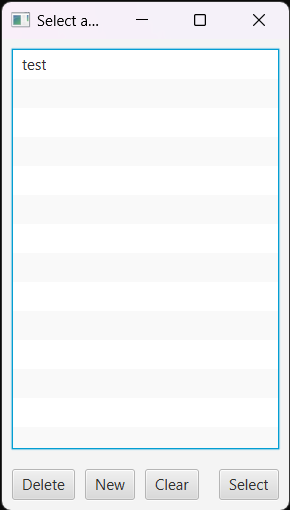
\includegraphics{database} \\
When you start the program, a small database menu will pop up to allow you to pick a database to store your code sequences 
using sqlite. 

In the image above, the "test" database is already created. If a database has not been created yet, 
then click on "New" to create a new one. 

After creation, to open it, click on that database and then "Select" to use that database.

"Delete" will simply create a database completely, while "Clear" will clear all the contents stored in that database.
\section{Main interface}
\subsection{Section categorization}
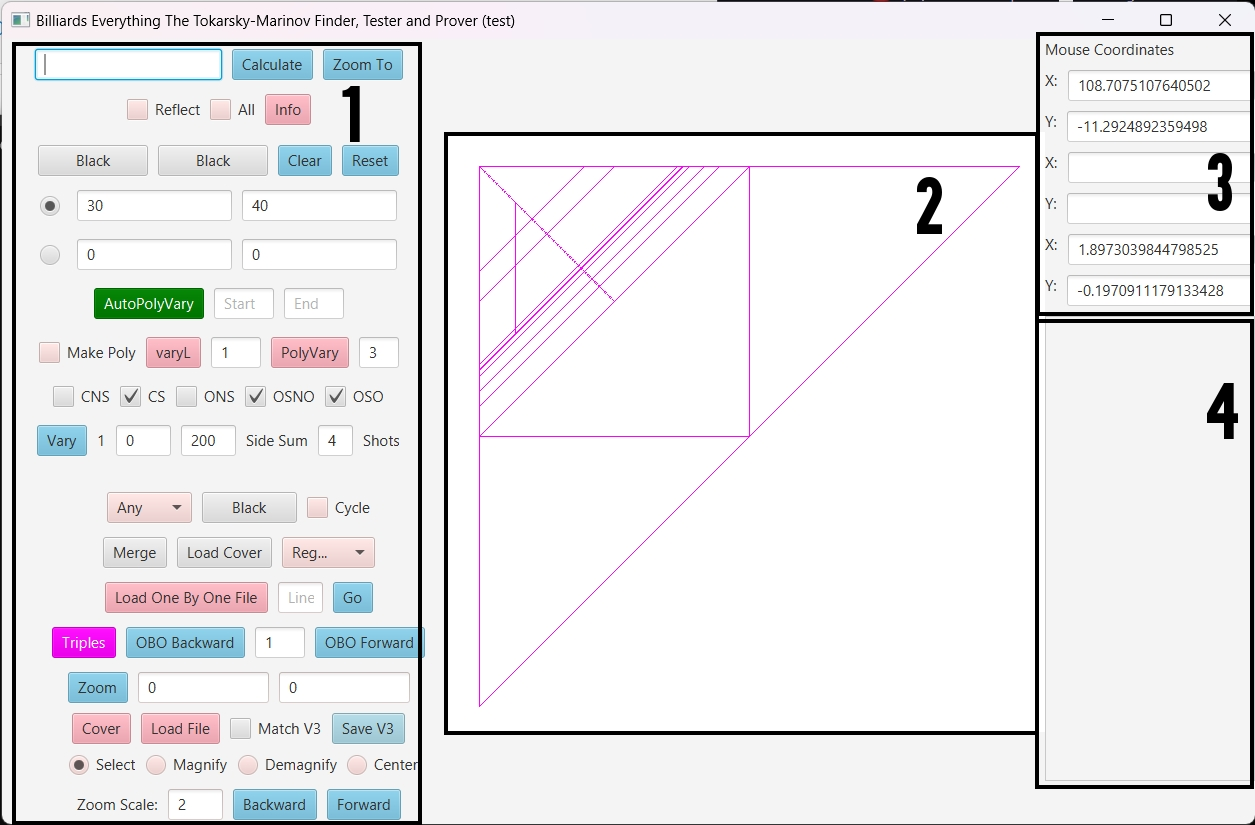
\includegraphics[scale = 0.38]{main_interface}
\begin{enumerate}[1 -]
  \item Tools: What you can do in this program
  \item Viewer: Show results
  \item Mouse coordinates: Show your mouse coordinates
  \item Code sequences: Show the code sequences
\end{enumerate}
\subsection{Tools}
In this section, we will focus on what each button do in the tools section. \\ 
\linebreak
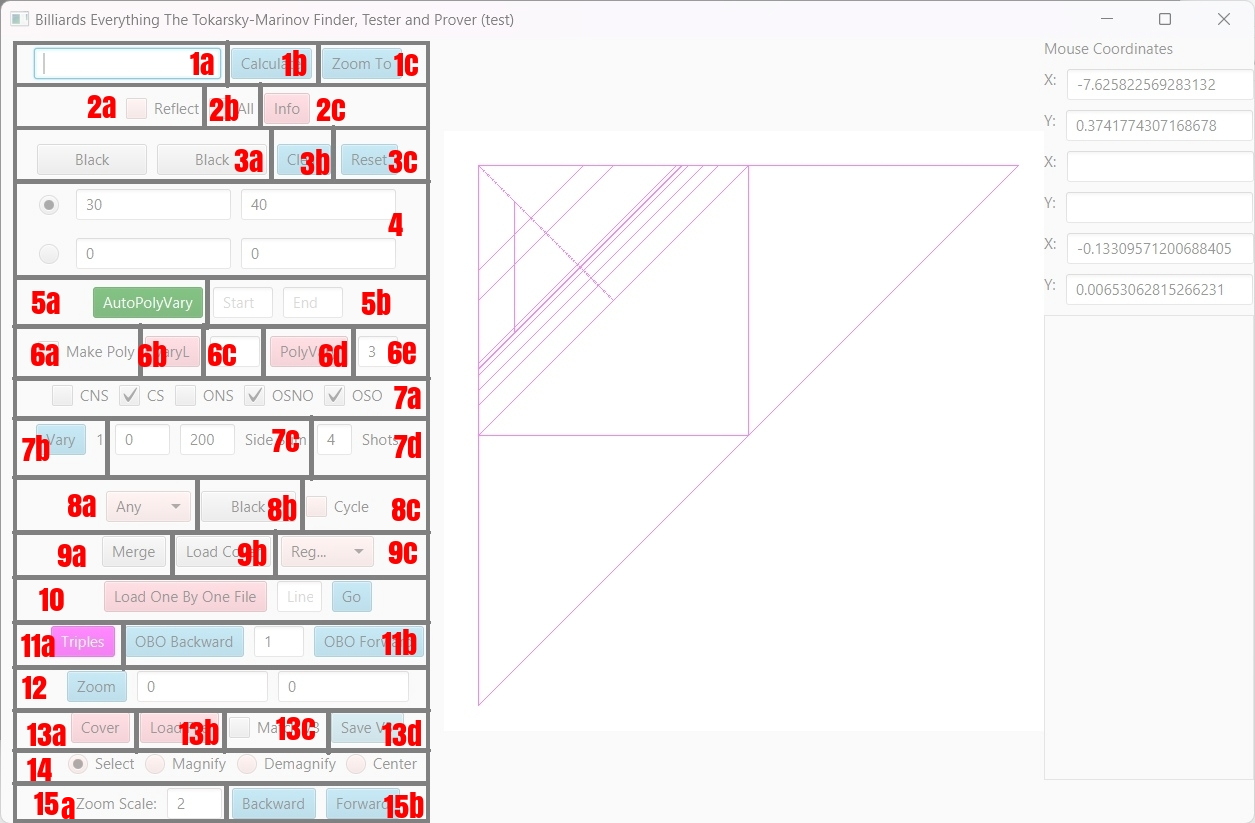
\includegraphics[scale=0.38]{main_interface_labeled}
\begin{enumerate}
  \item
  \begin{enumerate}[a.]
    \item Code seqence Box(triples require commas)
    \item Calculate Using Code Sequence, when clicked the \hyperref[iterwin]{Iteration Window} will appear 
    \item Zoom The Code Sequence
  \end{enumerate}
  \item 
  \begin{enumerate}[a.]
    \item Reflect the Viewer
    \item Permutes x,y,z coordinates
    \item Information about the Code Inputted
  \end{enumerate}
  \item 
  \begin{enumerate}[a.]
    \item Colour of the Regions in Viewer
    \item Clears Viewer
    \item Resets to Default
  \end{enumerate}
  \item  X Y Coordinates 
  \item 
  \begin{enumerate}[a.]
    \item Autopolyvary
    \item start end Autopolyvary
  \end{enumerate}
  \item 
  \begin{enumerate}[a.]
    \item Creates Polygon Vertices Coordinates 
    \item List of Coordinates
    \item Maximum Number of Regions Drawn From Coordinates of VaryL
    \item Polygon Coordinates
    \item Maximum Number of Subdivisions
  \end{enumerate}
  \item 
  \begin{enumerate}[a.]
    \item Code type
    \item Finds Codes and the number represents the Number of Codes Found after done
    \item Min Max Side Sum 
    \item Number of Shots
  \end{enumerate}
  \item 
  \begin{enumerate}[a.]
    \item  Total Number of Selected Polygons
    \item Colour of Cover Squares
    \item Cycles the Colours in the Cover

  \end{enumerate}
  \item 
  \begin{enumerate}[a.]
    \item Merges Abutting Covers
    \item Loads a Previous Cover
    \item Draws Selected Bounding Polygon
  \end{enumerate}
  \item  Load One By One File
  \item 
  \begin{enumerate}[a.]
    \item Triples, when clicked the \hyperref[triwin]{Triple Window} will appear
    \item Direction of One By One
  \end{enumerate}
  \item  Center the Viewer at the Coordinates
  \item 
  \begin{enumerate}[a.]
    \item Cover a Polygon with Stables and Triples, when clicked the \hyperref[covwin]{Cover Window} will appear
    \item Draws Codes From a Selected File
    \item Find Intersecting Code From ClickedLocation
    \item Save Code
  \end{enumerate}
  \item Select and Press on Viewer
  \item 
  \begin{enumerate}[a.]
    \item Zoom Times Size
    \item Undo Redo Viewer
  \end{enumerate}
\end{enumerate}
\section{Iteration Window}\label{iterwin}
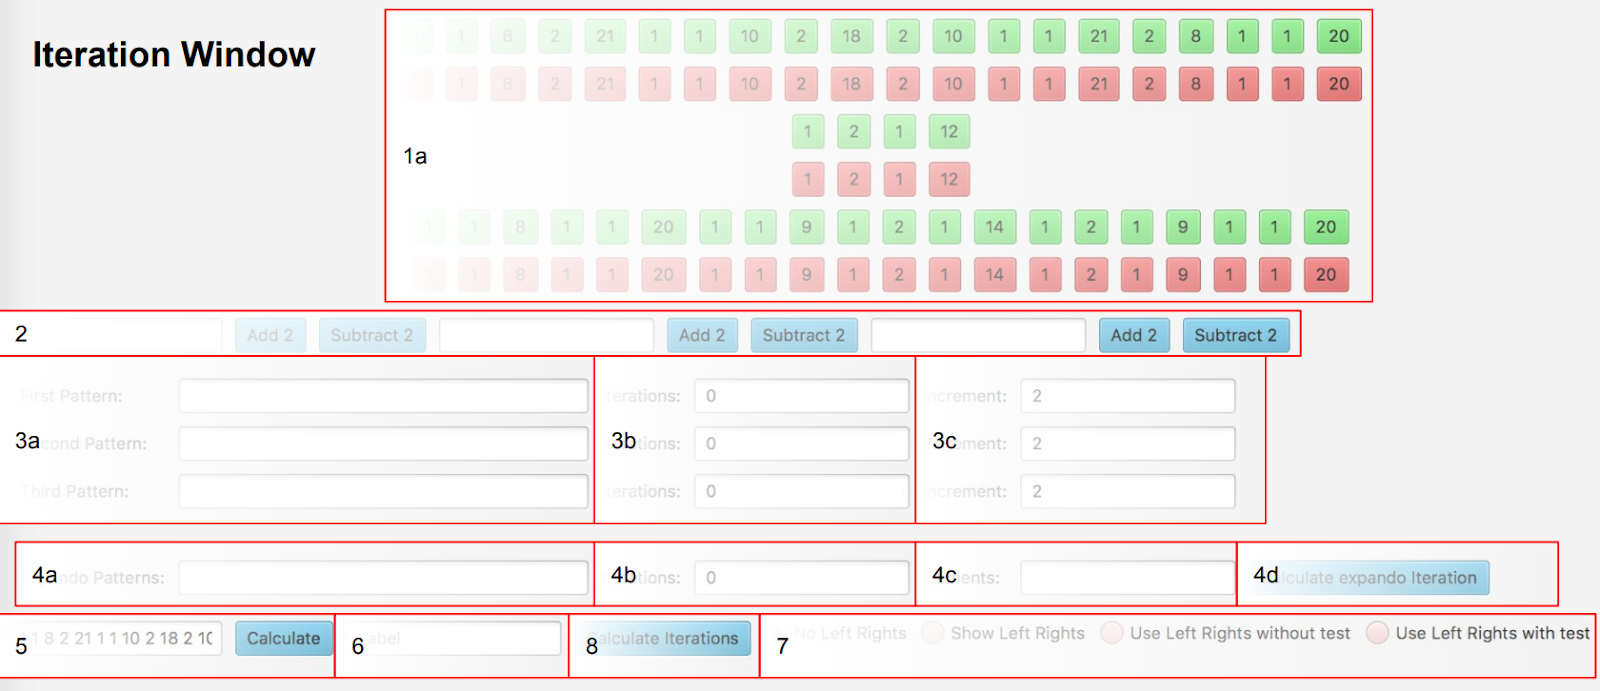
\includegraphics[scale=0.23]{iteration_window}
\begin{enumerate}
  \item
  \begin{enumerate}[a.]
    \item Increase/Decrease code Individually By 2
  \end{enumerate}
  \item Add 2/Subtract 2 at specified positions (for triples separate by comma)
  \item
  \begin{enumerate}[a.]
    \item Put in specified positions (for triples separate by comma)
    \item Put in specified number of iterations
    \item Put in specified increment
  \end{enumerate}
  \item
  \begin{enumerate}[a.]
    \item Put in valid horizontal pattern code
    \item Put in specified number of iterations
    \item Put in specified pattern of each element
    \item Press Button to calculate expando iterations
  \end{enumerate}
  \item Code Sequence Box (triples require commas)
  \item Label (Not required)
  \item Options for the iterations (read instructions)
  \item Calculate iterations using 3 and 7
\end{enumerate}
\section{Cover}\label{covwin}
In Cover, you want to have a polygon, which is the region you want to cover it completely with periodic paths, hence the name Cover.
\\ \\
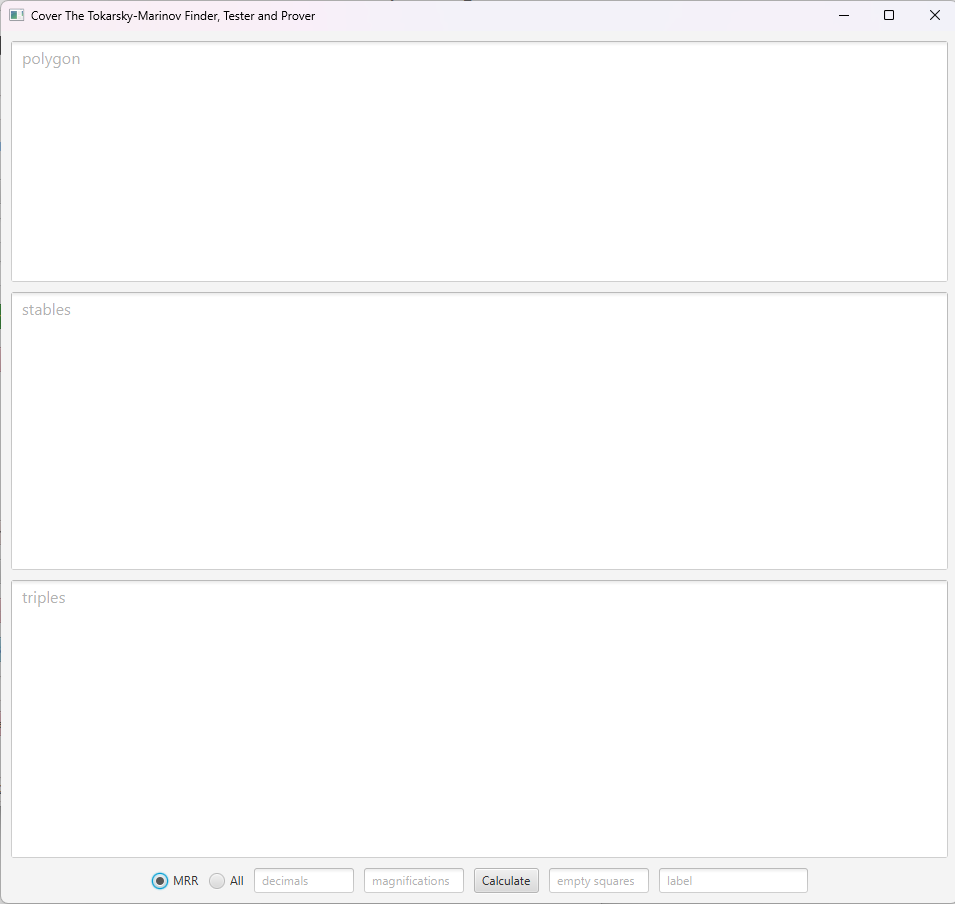
\includegraphics[scale=0.5]{cover_window}
\begin{itemize}
  \item Polygon: the area you want to cover, for example
  
  5 5

  5 6

  6 5

  is the area of the triangle with those 3 vertices.
  \item Stables: side sequences that cover some part of the region
  \item Triples: triples that cover some part of the region
  \item MRR/All: Choosing the all options from the radio button to find all equations including the MRR equations and guarantees every square will satisfy the gradient algorithm.
  \item decimals: how accurate you want to be
  \item magnification: square division
  \item Calculate button: start covering the region with the code you put in stables and triples.
  \item empty squares: the number of empty squares that you are looking to find
  \item label: label your progress
\end{itemize}
\section{Triple Window}\label{triwin}
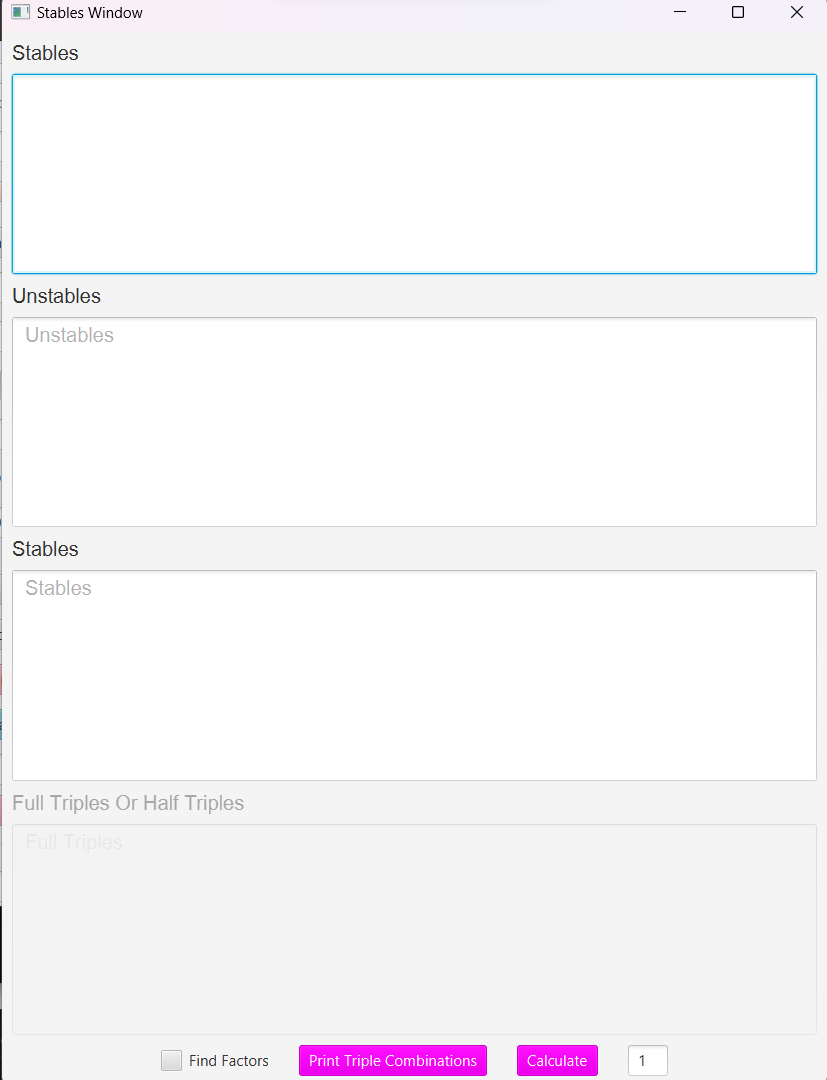
\includegraphics[scale=0.6]{triple_windows}

The triple window will pair up 2 stables with 1 unstables to find a triple.
\section{VaryL Window}\label{varyL}
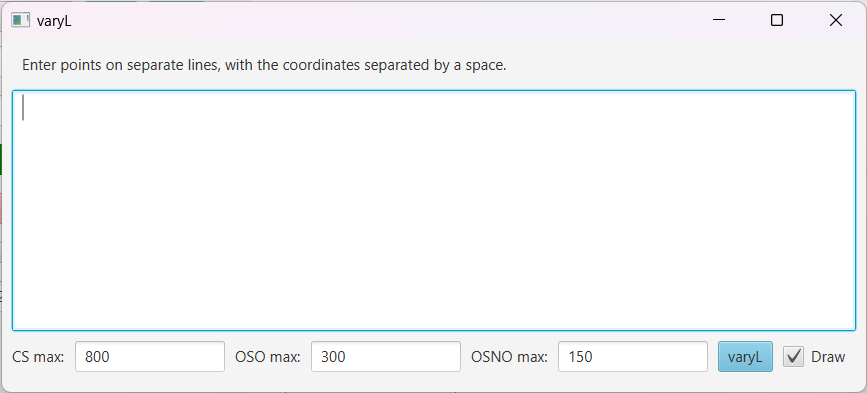
\includegraphics[scale=0.75]{varyL}
To run AutoPolyVary, you first have look at \hyperref[covers]{this}. 
You will see a set of coordinates after pressing Calculate. 
Copy those coordinates into the box and press the varyL button as the program will run vary on all those coordinates.
\section{AutoPolyVary Window}\label{AutoPolyVary}
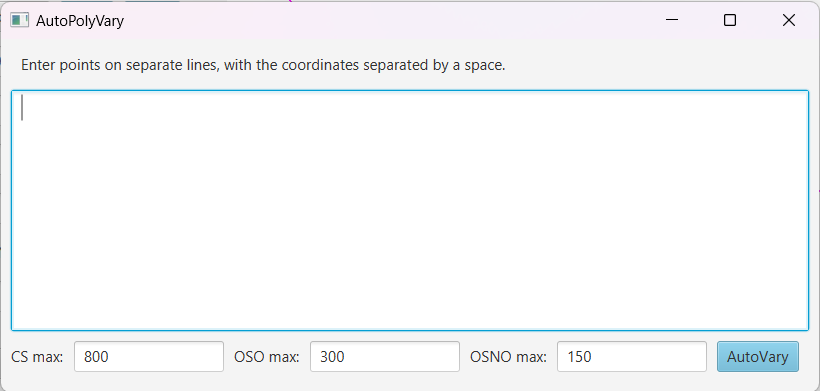
\includegraphics[scale=0.75]{Autopolyvary}
To run AutoPolyVary, you first have to look at \hyperref[covers]{this}. 
You will see a set of coordinates after pressing Calculate. 
Put those coordinates in an empty file and then use "Load one by one file" in the tools menu to load that file. 
Then you need to put the same polygon you were using in \hyperref[cover_window]{Cover Windows} into the window and press AutoVary as the program run PolyVary on all the coordinates in the file.

\chapter{How to be a periodic path hunter}
This chapter will assume you have contacted George Tokarsky. He will give you a coordinates so that 
you can find the perdiodic path in the given space.
\section{Identify your given open space}\label{id}
\begin{enumerate}[Step 1.]
  \item Your polygon (or quadrilateral) coordinates will be given as below when you contacted George Tokarsky or you can just create one independently, they are the coordinates of the vertices of your polygon. For example:

  8 58
  
  9 57
  
  9 55
  
  8 56
  
  \item Now go to the tools menu and click on "Cover" in the bottom left region. These polygon coordinates should then be copied and pasted into the first big input box with the hint "Polygon". This is the first of three big input boxes titled polygon, stables, triples. 
  \item Look towards the bottom of the Cover pop-up and make sure MRR is selected and use these suggested
  numbers as follows 22 20 [Calculate] 50 respectively. 

  Calculate is used to outline your polygon and to find uncovered holes in the viewer. The 3 numbers
  around the calculator button are specifications.
  
  First small box is the number of decimal places, which you do not need to change. 
  
  Second small box is the number of subdivisions, which you may need to change or increase towards the end of
  covering the polygon. 

  Third small box is the list of point coordinates displayed where those points are not covered. Generally
  50-100 points is good enough for a single session to start.
  Eventually you will need to use thousands of points and leave the program run overnight or longer.
\end{enumerate}

\section{Filling in spaces/hole (Stables)}
There are many ways of filling empty space. 
The possible ways of filling spaces will be loosely ordered by the size of the holes to fill. \\
Most values, such as subdivisions and side sum or code sum are dependent on your processor specs. 
Loose ranges and example values will be called low, medium or high and will be specified in the steps below.
Here, we will introduced severeal tools to fill in spaces/hole
\subsection{Menu - PolyVary}
Generally used for a new polygon. 
\begin{enumerate}[Step 1.]
  \item Subdivision should be set to a low-medium range (3 - 5). 
  \item Side sum should be of medium range (800 - 1200). 
  \item CS should be selected first.
  \item Do not forget to change your number of cores beside "Shots".
  \item Click on PolyVary and put in the given polygon coordinates appearing there and press the Vary button 
  seen inside.
  \item Copy all code sequences that show up in the console.
  \item Paste these code sequences into the second big input box under Cover (if it is empty then there will be a
  hint text that says stables.)
\end{enumerate}

  Note: Increasing the subdivisions, side sum or code sum can help find smaller holes, as well as zooming to
enlarge the viewer with empty space which can help to find more
code sequences but in return will take longer.
\subsection{Menu - Side Sum}
When the side sum is over 1000 or so, it could be time to increase your point coordinates into the
thousands. 
\begin{enumerate}[Step 1.]
  \item Put your coordinate list inside varyL and press the varyL button inside.
  \item Make sure that you check the box on Draw. 
  
  Note: the max boxes are in code sums not side sums. 
  
  A typical start is CS max 333 and increase that as needed up to the 500's.

  For the OSO max use a range of 122-166 or so and for the OSNO use a range of 50-136 or so. 

  Caution:
  The checkboxes in the Tools Menu should be on for the CS first, then with the CS and OSO on and then
  lastly with the CS,OSO and OSNO on.
\end{enumerate} 




\subsection{Menu - Match V3/Save V3}
This tool can be used to find holes individually. It should be used when almost finished with the cover but can be used whenever the user likes to.
\begin{enumerate}[Step 1.]
  \item Side sum should be set to between 2000 to 5000
  \item Make sure that CS is the only code type selected as the other two types take much more time. 
  \item Zoom in enough to see the hole.
  \item Make sure Match V3's checkbox is checked. Click Select as the radio option.
  \item Click on the corners of the given empty space on the viewer. Match V3 will find the common sequences
  of all the coordinates clicked on the viewer.
  \item Next, check the console for something similar: \\
  //---------------------- Matching Code Sequences ----------------------//

  CS (56, 384) 1 1 6 2 20 2 9 1 2 1 19 2 8 2 19 1 2 1 9 2 20 2 6 1 1 19 2 8 2 20 2 8 2 20 2 7 1 3 20 2 8 2 20
  3 1 7 2 20 2 8 2 20 2 8 2 19

  CS (88, 412) 1 1 4 1 1 18 1 1 4 1 1 18 1 1 4 1 1 18 1 1 4 1 1 18 1 1 4 1 1 18 1 2 1 10 1 2 1 19 3 1 7 2 19
  1 2 1 10 1 2 1 18 1 2 1 10 1 2 1 18 1 2 1 10 1 2 1 18 1 2 1 10 1 2 1 19 2 7 1 3 19 1 2 1 10 1 2 1 18

  ...
  \item Copy a single code sequence and put it in the sequence drawer and click on "Calculate". 
  
  If the code sequence covers what you wish it to cover, 
  then put it in the "Stables" input box in Cover(second input box). 

  If it does not cover what you wish, you can either try the next matching sequence or you can keep the
  sequences and repeat this process for the smaller empty space.
  
  Alternatively you can also save them all together in any file you choose by pressing Save V3 and load
  
  them all when ready by pressing the load button.
  
  If the hole looks like a line, you can click on both sides of the line to see if there is any matching code
  
  sequences. You can also try using a triple below.
\end{enumerate}







\section{Filling in spaces/holes (triples)}

These holes are very long rectangles that look like lines. A triple is just a combination of stable, unstable, stable codes.

Example of a triple with commas:

1 1 10 2 23, 1 2 1 13 2 20 2 13, 1 1 12 2 20 2 13 1 2 1 13 2 20 2 12 1 1 23 2 12 2 20 2 12 2 23

To find the two stables, click one side of the line and then the other side and you should get the two stables as long as they intersect in a common boundary line.

To find the unstable involves loading low side sum (100 should be good enough) CNS and ONS and

connecting the existing sequences to the left and right of the CNS/ONS sequence found.

To find the unstable use the two radio buttons next to the two rows of coordinates near the top in the Tools

Menu.

1. Click on the first radio button and click on one end of the line (a close approximation is all you need)

and its coordinates will appear.

2. Click on the second radio button and click on the other end of the line and its coordinates will appear.

3. Change the Side Sum to 144 or so and only have the CNS and ONS check boxes selected.

4. Press Vary and you will see a list of unstables in the console.

5. Copy all the code sequences found into a text file which we will call lines.txt

6. Click "Load File". Find and click on lines.txt. (some will say empty and others don't work).

7. Go back to the viewer and click anywhere on the given line. Find any CNS or ONS that appears in the

Coordinate/Codes Column underneath the coordinates.

If none appears, try again with a bigger Side Sum and more shots. Hopefully you will find one and you

can take the first unstable in the list.

Now go to the Tools Menu under Cover, paste the sequence stable, unstable, stable in the third input box

as with the example and with the hint triples.

To double check you can copy the triple sequence into the box next to Calculate in the Tools Menu to see

if the line has been filled or partially.

Alternatively if using a triple, you can try using a stable OSO or OSNO to cover that line.

\section{Finding more holes to fill}\label{covers}
After following \hyperref[id]{Identify your given open space}. 
\begin{enumerate}[Step 1.]
  \item Go to "Cover" in the bottom left of the tools menu and click on the Calculate button
  \item Go to the console. Within the generated text should be something similar
  
  1653711 stable squares used in the cover

  0 triple squares used in the cover
  
  2310 stables used in the cover
  
  0 triples used in the cover
  
  MRR at 22 decimals, deepest magnification 27
  
  Total stable cost: 831208131
  
  485334 squares were not filled in
  
  8.2754087448120117 57.724614143371582
  
  8.2933473587036133 57.561535835266113
  
  ...
  
  Not Covered
  
  Time elapsed: 22m 20.514s
  \item Copy all pairs of coordinates and paste into an accessible text file.
  \item From the Tools Menu, go to "Load One By One File" and choose the text file that contains all the copied
  coordinates. The viewer will automatically move to the first coordinate in the text file.
  To go to the next pair of coordinates, click on "OBO Forward". Repeat filling the holes until the given
  polygon is covered.
  When done the console should say "Covered" like this:

  // 0 squares were not filled in

  // 1111 stable squares used in the cover

  // 24 triple squares used in the cover

  // 31 stables used in the cover

  // 2 triples used in the cover

  // MRR at 7 decimals, 1x1 number of squares, deepest magnification 17

  // Total stable cost: 65809

  // Covered

  // Time elapsed: 0.128s

  Note: you can used \hyperref[AutoPolyVary]{AutoPolyVary} as well as \hyperref[varyL]{VaryL} to do the steps automatically.
\end{enumerate}

\section{What should a great periodic path hunter do next}
Go to the jar called Billiards Everything and you will find a folder called Cover. Send that to me and I
  will check it and run it to the All proof that goes through all the equations and we will add your name,
  date and cover to the Great Hunt. You can do that yourself if you wish by checking the All check box
  instead of the MRR check box. If you do, be prepared that it could take 20 times or more and days or
  weeks or months or years. To ensure that the polygon assigned is full look for two things:

  // 0 squares were not filled in
  
  // 1111 stable squares used in the cover
  
  // 24 triple squares used in the cover
  
  // 31 stables used in the cover
  
  // 2 triples used in the cover
  
  // MRR at 7 decimals, 1x1 number of squares, deepest magnification 17
  
  // Total stable cost: 65809
  
  // Covered
  
  // Time elapsed: 0.128s \\
This shows that your polygon is covered and I will run the proof to ensure that the polygon has been fully
covered.


\section{Bonus fun on iterations}
\subsubsection{Iteration}
When you put in a code which can be a stable, a non-stable or a triple and press Calculate, the iterations
bar comes up.

If you use a triple, you will see six rows of boxes, three green and three pink. Otherwise you will see two
rows of boxes. Pressing a green increases the code by two and pressing the pink decreases the code by
two.

Alternatively you can use the Add 2/Subtract 2 boxes to change a given code. In the empty box to the left,
if you put in for example 3 6 10 then the 3rd, 6th and 10th code number will add 2 or subtract 2 to those
spots. 

Similarly for triples if you put in 3, 2, 3 5 and press add 2 it will add 2 to the 3rd spot of the first
stable, add 2 to the 2nd spot of the unstable and add 2 to the 3rd and 5th spots of the other stable.

You can also create patterns using the next three horizontal lines of boxes. For example using the First
Pattern box and putting in 3 6 10 for those spots, and putting 12 in the second box will give the number of
iterations and putting 6 in the third box will give the increment to all of those spots. Then press the button
Calculate Iterations and you will see in the viewer all those regions belonging to all of those codes.

Furthermore, there are also four options you can choose from for calculating iterations:

First is the ‘no left rights’ option which means it doesn't use any previous left rights equations in the
calculation for the following iterations, and then each time it calculates and uses the current left rights
equations which will take the longest time.

The second is ‘show left rights' which does the same as the first but will also print out the left rights for
each code in the iterations in the console.

The third option is ‘use left rights without test’ which means using the left rights found in the previous
iterations in the calculation for the following iterations and thus it does NOT always give you the correct
result. The trade off is if you trust the pattern, then this is the fastest option.

The last option is ‘use left rights with test’ which means using left rights found in the previous iteration in
the calculation for the following iterations with a test. This test can filter out many wrong results and then
use the normal method to calculate instead. It is the second-fastest option but again is not foolproof.

NOTE: the third and the fourth option works with only the stable codes and doesn't work for the unstable
codes.
\subsubsection{Expando Iterations}
Expando iterations are used when the code sequences expand horizontally in a pattern and where the left
rights of the code sequences also have a pattern. Here is an example:

1 1 2 2 1 1 3 3

1 1 2 2 2 2 1 1 3 2 2 3

1 1 2 2 2 2 2 2 1 1 3 2 2 2 2 3

...
Left Right

(2, 0, 7, 0)

(8, 0, 5, 0)

(8, 0, 1, 0)

(4, 0, 1, 0)

Left Right

(2, 0, 9, 0)

(10, 0, 7, 0)

(10, 0, 1, 0)

(4, 0, 1, 0)

Left Right

(2, 0, 11, 0)

(12, 0, 9, 0)

(12, 0, 1, 0)

(4, 0, 1, 0)

...

To use and press the Calculate expando iteration button, put in the expando pattern box a pattern
substituted with the capital letters.

For example input 1 1 2 2 A 1 1 2 2 B 1 1 2 2 A in the Expando pattern box and put in the elements box
for example: 2 2,2 2 separated by commas with A becomes 2 2 and B becomes 2 2. This also allows
expanding patterns involving A,B,C,...

The Expando iteration has only two options to use:

a. use 'left rights with test’ means all the code sequences in the iterations are calculated the normal way
which is the slower method and this acts as the test.

b. use 'left rights without test’ means using the left rights found in the previous iteration in the calculation
for the following iterations. Again this is not foolproof
\end{document}